% F049: native TikZ/PGFPlots, computed from the stated mathematical model.
\begin{center}
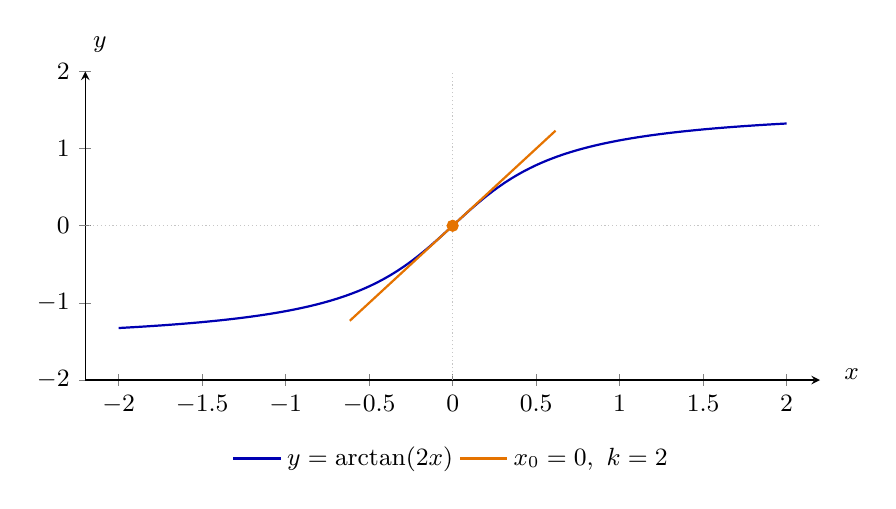
\begin{tikzpicture}[font=\small,>=stealth]
\begin{axis}[width=.90\linewidth,height=5.5cm,xmin=-2.2,xmax=2.2,ymin=-2,ymax=2,
axis lines=left,xlabel={$x$},ylabel={$y$},font=\small,
xlabel style={at={(axis description cs:1.02,.02)},anchor=west},
ylabel style={rotate=-90,at={(axis description cs:.02,1.03)},anchor=south},
legend style={at={(axis description cs:.5,-.18)},anchor=north,draw=none,fill=none,font=\small,legend columns=2},
unbounded coords=jump,clip=true,]
\addplot[gray!45,thin,densely dotted,forget plot] coordinates {(-2.2,0) (2.2,0)};
\addplot[gray!45,thin,densely dotted,forget plot] coordinates {(0,-2) (0,2)};
\addplot[blue!70!black,thick] coordinates {(-2,-1.3258177) (-1.9777778,-1.3231757) (-1.9555556,-1.3204773) (-1.9333333,-1.3177207) (-1.9111111,-1.314904) (-1.8888889,-1.3120254) (-1.8666667,-1.3090828) (-1.8444444,-1.3060741) (-1.8222222,-1.3029971) (-1.8,-1.2998495) (-1.7777778,-1.2966289) (-1.7555556,-1.2933328) (-1.7333333,-1.2899586) (-1.7111111,-1.2865036) (-1.6888889,-1.2829649) (-1.6666667,-1.2793395) (-1.6444444,-1.2756244) (-1.6222222,-1.2718162) (-1.6,-1.2679115) (-1.5777778,-1.2639067) (-1.5555556,-1.259798) (-1.5333333,-1.2555816) (-1.5111111,-1.2512533) (-1.4888889,-1.2468086) (-1.4666667,-1.2422432) (-1.4444444,-1.237552) (-1.4222222,-1.2327302) (-1.4,-1.2277724) (-1.3777778,-1.222673) (-1.3555556,-1.2174261) (-1.3333333,-1.2120257) (-1.3111111,-1.206465) (-1.2888889,-1.2007373) (-1.2666667,-1.1948354) (-1.2444444,-1.1887515) (-1.2222222,-1.1824776) (-1.2,-1.1760052) (-1.1777778,-1.1693253) (-1.1555556,-1.1624283) (-1.1333333,-1.1553042) (-1.1111111,-1.1479424) (-1.0888889,-1.1403316) (-1.0666667,-1.1324598) (-1.0444444,-1.1243144) (-1.0222222,-1.1158821) (-1,-1.1071487) (-0.97777778,-1.0980992) (-0.95555556,-1.0887176) (-0.93333333,-1.0789872) (-0.91111111,-1.0688899) (-0.88888889,-1.0584069) (-0.86666667,-1.047518) (-0.84444444,-1.036202) (-0.82222222,-1.0244363) (-0.8,-1.012197) (-0.77777778,-0.99945885) (-0.75555556,-0.98619507) (-0.73333333,-0.97237743) (-0.71111111,-0.95797612) (-0.68888889,-0.94295973) (-0.66666667,-0.92729522) (-0.64444444,-0.9109479) (-0.62222222,-0.89388147) (-0.6,-0.87605805) (-0.57777778,-0.85743823) (-0.55555556,-0.83798123) (-0.53333333,-0.81764505) (-0.51111111,-0.79638673) (-0.48888889,-0.77416268) (-0.46666667,-0.75092906) (-0.44444444,-0.72664234) (-0.42222222,-0.70125992) (-0.4,-0.67474094) (-0.37777778,-0.64704719) (-0.35555556,-0.61814423) (-0.33333333,-0.5880026) (-0.31111111,-0.55659932) (-0.28888889,-0.52391935) (-0.26666667,-0.48995733) (-0.24444444,-0.45471927) (-0.22222222,-0.41822433) (-0.2,-0.38050638) (-0.17777778,-0.34161549) (-0.15555556,-0.30161905) (-0.13333333,-0.26060239) (-0.11111111,-0.21866895) (-0.088888889,-0.17593963) (-0.066666667,-0.13255153) (-0.044444444,-0.088655882) (-0.022222222,-0.044415215) (0,0) (0.022222222,0.044415215) (0.044444444,0.088655882) (0.066666667,0.13255153) (0.088888889,0.17593963) (0.11111111,0.21866895) (0.13333333,0.26060239) (0.15555556,0.30161905) (0.17777778,0.34161549) (0.2,0.38050638) (0.22222222,0.41822433) (0.24444444,0.45471927) (0.26666667,0.48995733) (0.28888889,0.52391935) (0.31111111,0.55659932) (0.33333333,0.5880026) (0.35555556,0.61814423) (0.37777778,0.64704719) (0.4,0.67474094) (0.42222222,0.70125992) (0.44444444,0.72664234) (0.46666667,0.75092906) (0.48888889,0.77416268) (0.51111111,0.79638673) (0.53333333,0.81764505) (0.55555556,0.83798123) (0.57777778,0.85743823) (0.6,0.87605805) (0.62222222,0.89388147) (0.64444444,0.9109479) (0.66666667,0.92729522) (0.68888889,0.94295973) (0.71111111,0.95797612) (0.73333333,0.97237743) (0.75555556,0.98619507) (0.77777778,0.99945885) (0.8,1.012197) (0.82222222,1.0244363) (0.84444444,1.036202) (0.86666667,1.047518) (0.88888889,1.0584069) (0.91111111,1.0688899) (0.93333333,1.0789872) (0.95555556,1.0887176) (0.97777778,1.0980992) (1,1.1071487) (1.0222222,1.1158821) (1.0444444,1.1243144) (1.0666667,1.1324598) (1.0888889,1.1403316) (1.1111111,1.1479424) (1.1333333,1.1553042) (1.1555556,1.1624283) (1.1777778,1.1693253) (1.2,1.1760052) (1.2222222,1.1824776) (1.2444444,1.1887515) (1.2666667,1.1948354) (1.2888889,1.2007373) (1.3111111,1.206465) (1.3333333,1.2120257) (1.3555556,1.2174261) (1.3777778,1.222673) (1.4,1.2277724) (1.4222222,1.2327302) (1.4444444,1.237552) (1.4666667,1.2422432) (1.4888889,1.2468086) (1.5111111,1.2512533) (1.5333333,1.2555816) (1.5555556,1.259798) (1.5777778,1.2639067) (1.6,1.2679115) (1.6222222,1.2718162) (1.6444444,1.2756244) (1.6666667,1.2793395) (1.6888889,1.2829649) (1.7111111,1.2865036) (1.7333333,1.2899586) (1.7555556,1.2933328) (1.7777778,1.2966289) (1.8,1.2998495) (1.8222222,1.3029971) (1.8444444,1.3060741) (1.8666667,1.3090828) (1.8888889,1.3120254) (1.9111111,1.314904) (1.9333333,1.3177207) (1.9555556,1.3204773) (1.9777778,1.3231757) (2,1.3258177)};
\addlegendentry{$y=\arctan(2x)$}
\addplot[orange!90!black,thick] coordinates {(-0.616,-1.232) (0.616,1.232)};
\addlegendentry{$x_0=0,\ k=2$}
\addplot[only marks,mark=*,orange!90!black,forget plot] coordinates {(0,0)};

\end{axis}
\end{tikzpicture}
\par\smallskip{\small 按本题原函数绘图；切线斜率由本题的导函数计算。}
\end{center}
